\documentclass[Rapport/Rapport_main.tex]{subfiles}
\begin{document}
\subsection{Grænseflader}\label{sec:rap_interfaces}
I dette afsnit beskrives kommunikationsprotokollerne mellem de forskellige enheder. Systemet gør brug af I2C protokollen, hvor RPi'en er 'Master' og PSoC enhederne er 'slaves'. For den fulde dokumentation se \textbf{Arkitektur} \fullref{arch:sec:protocols}.
\subsubsection{Kommunikation mellem Rasberry Pi Zero W og PSoC enheder}
Playerside, BallDispenser og RPi enhederne er alle tilkoblet til samme I2C-bus. For I2C kommunikation gælder: 
\begin{itemize}
    \item Clock speed : 100 kbits / s 
\end{itemize}
\textbf{Protokolstruktur}
\begin{figure}[H]
    \centering
    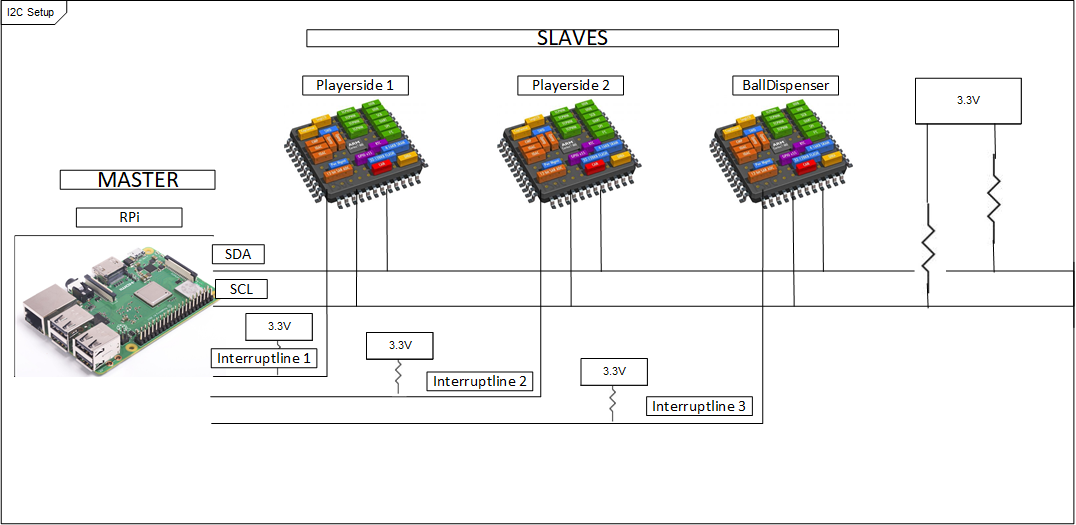
\includegraphics[width=\textwidth]{Rapport/Arkitektur/graphics/I2C-Illustration.png}
   \caption{Skitse af I2C kommunikation. Kommunikationen mellem enhederne starter enten med at RPi'en (MASTER) ønsker at sende data til Playerside eller BallDispenser (SLAVES) eller hvis en af slaverne sender et interrupt (Trækker interruptlinje lavt).}
    \label{fig:sketch_interrut}
\end{figure}
Figur \ref{fig:sketch_interrut} viser en visuel repræsentation af kommunikationopbygningen. Interruptlinen er aktiv lav - da alt kommunikation skal initieres af 'Master'-enheden, trækker PSoC-enhederne interruptlinjen lavt, for at indikere de har nyt data. Efter dataen er læst trækkes interruptlinjen højt igen
\begin{table}[H]
    \centering
    \begin{tabular}{|L{0.2\textwidth}|L{0.15\textwidth}|L{0.15\textwidth}|L{0.15\textwidth}|L{0.15\textwidth}|}
\hline
\textbf{Bit 0 - 6} & \textbf{Bit 7} & \textbf{Bit 8} & \textbf{Bit 9 - 16}  & \textbf{Bit 17} \\ \hline
Slave Address & R/W & ACK & Data Bit & NACK \\ \hline
\end{tabular}
    \caption{Eksempel på I2C kommunikation. Bit 9 - 16 er det data som ønskes at sendes. Den er i dette eksempel repræsenteret som en byte, men der kan sendes flere, hvis det ønskes.}
\end{table}

\subsubsection{Kommunikation mellem RPi og Playerside}
Playersides skal registere antal kopper tilbage på de angivede pladser. Denne information er vital for RPi’en, som videregiver denneinformation til andre delsystemet (fx Display og WebPage). Playerside sender ét byte til RPi, hvor de 6 LSB bit repræsenterer en kop. Et højt bit betyderat en kop er placeret på den angivet plads, se figur \ref{fig:cups_setup}.
\begin{figure}[H]
    \centering
    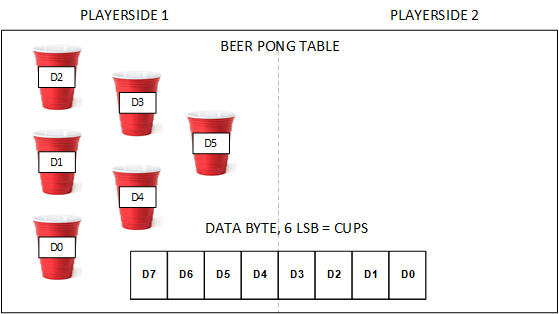
\includegraphics[width=\textwidth]{Arkitektur/Grenseflader/Graphics/cups.png}
    \caption{Repræsentation af 1 byte af kopper}
    \label{fig:cups_setup}
\end{figure}
For den fulde dokumentation henvises til afsnittet \fullref{arch:sec:RPi_Playerside_com} i bilaget \textbf{Arkitektur} \fullref{arch:sec:protocols}.
\subsubsection{Kommunikation mellem RPi og BallDispenser}
RPi sender diktere hvilke tilstande BallDispenser-enheden skal instantiere, og BallDispenser sender hvilke events som opstår for systemet: Ingen bolde, Bolde eller Møntindkast. For den fulde dokumentation henvises til afsnittet "Grænseflade mellem RPi og BallDispenser" i \textbf{Arkitektur} afsnit \fullref{arch:sec:protocols}.

\end{document}